\documentclass[12pt,a4paper]{jsarticle}
\usepackage[utf8]{inputenc}
\usepackage[japanese]{babel}
\usepackage{amsmath}
\usepackage{amsfonts}
\usepackage{amssymb}
\usepackage{graphicx}
\usepackage{url}
\usepackage{listings}
\usepackage{xcolor}
\usepackage{geometry}
\usepackage{fancyhdr}
\usepackage{booktabs}
\usepackage{array}
\usepackage{longtable}
\usepackage{here}

% ページ設定
\geometry{left=25mm,right=25mm,top=30mm,bottom=30mm}

% ヘッダー・フッター設定
\pagestyle{fancy}
\fancyhf{}
\fancyhead[L]{システム統合レポート}
\fancyhead[R]{\thepage}
\renewcommand{\headrulewidth}{0.4pt}

% タイトル情報
\title{プログラミング応用 最終課題レポート\\
\large 新システム提案・計画書}
\author{
グループ名:グループ13 フル単\\
メンバー:井田 礼慈(学籍番号:35714012)\\
\quad\quad\quad 大橋 蒼一朗(学籍番号:35714026)\\
\quad\quad\quad 松岡 遼(学籍番号:35714128)\\
}
\date{\today}

\begin{document}

\maketitle

\newpage

\section{システムの概要}
手話を自然な日本語で読み上げるシステム。手話の映像からAIによって意味を識別し、自然な日本語に変換する。
\section{背景}

% 現在のシステムやプロセスにおける問題点を記述
聴覚障害者の主なコミュニケーション手段として手話と筆談があるが、手話の習得は難しく、手話が通じる人の数は少ない現状がある。


\section{目的}

% プロジェクトの全体的な目標を記述
聴覚障害者のコミュニケーションの障壁をなくし、聞き手に手話の知識がなくても、会話ができるようにすることを目的とする。

\section{実現上の課題}

\begin{itemize}
    \item 映像から単語への変換
    \item 単語列から自然な文章への変換
    \item 精度
\end{itemize}

\section{解決法}

\subsection{映像から単語への変換}
% 技術的課題に対する解決策を詳述
既存のLLMをもとに転移学習によって手話の映像から単語に変換するAIを作成する。
\subsubsection{単語列から自然な文章への変換}
% 提案するシステムのアーキテクチャを説明
既存のLLMを利用する。
\subsubsection{精度}
% データ統合の具体的手法を説明
画像認識に加え、専用のモーションキャプチャを行う手袋を作成し、利用することで精度を向上させる。\\
翻訳ミスをデータベースに記録し、一定期間の後、再度チューニングを行うことで地域差や個人差に適応する。\\
\subsubsection{セキュリティ対策}
% セキュリティに関する解決策を説明

\subsection{運用上の解決策}
% 運用面での解決策を詳述

\subsubsection{移行戦略}
% システム移行の戦略を説明

\subsubsection{ユーザーサポート体制}
% ユーザーサポートの体制を説明

\subsection{組織的解決策}
% 組織・人的課題に対する解決策を詳述

\section{実装工程表}

\subsection{プロジェクト全体スケジュール}
手話認識システムの開発を2026年4月から2027年8月まで(17ヶ月間)で実施する計画である。

\begin{longtable}{|p{3cm}|p{2.5cm}|p{6cm}|p{3cm}|}
\hline
\textbf{フェーズ} & \textbf{期間} & \textbf{主要作業} & \textbf{成果物} \\
\hline
\endhead

フェーズ1:企画・設計 & 2026年4月-7月 & 
\begin{itemize}
\item 要件定義
\item 基本設計
\item 詳細設計
\end{itemize} & 
\begin{itemize}
\item 要件定義書
\item 基本設計書
\item 詳細設計書
\end{itemize} \\
\hline

フェーズ2:AI開発 & 2026年8月-2027年2月 & 
\begin{itemize}
\item 手話データ収集
\item 画像認識AI開発
\item 自然言語変換開発
\item モーションキャプチャ技術開発
\end{itemize} & 
\begin{itemize}
\item 手話認識AIモデル
\item 自然言語変換モデル
\item モーションキャプチャシステム
\end{itemize} \\
\hline

フェーズ3:アプリ開発 & 2026年11月-2027年5月 & 
\begin{itemize}
\item UI/UX設計
\item フロントエンド開発
\item バックエンド開発
\item データベース構築
\end{itemize} & 
\begin{itemize}
\item ユーザーインターフェース
\item アプリケーション
\item データベースシステム
\end{itemize} \\
\hline

フェーズ4:テスト・導入 & 2027年3月-8月 & 
\begin{itemize}
\item 単体テスト
\item 統合テスト
\item ユーザーテスト
\item システム移行・導入
\end{itemize} & 
\begin{itemize}
\item テスト報告書
\item 運用システム
\item 運用マニュアル
\end{itemize} \\
\hline
\end{longtable}

\subsection{詳細マイルストーン}
\begin{enumerate}
    \item 要件定義完了:2024年5月
    \item 基本設計完了:2024年7月
    \item プロトタイプ完成:2024年10月
    \item β版リリース:2025年3月
    \item 本格運用開始:2025年8月
\end{enumerate}

\subsection{並行開発スケジュール}
\begin{table}[h]
\centering
\caption{開発チーム別スケジュール}
\begin{tabular}{|l|c|c|c|c|c|c|}
\hline
\textbf{チーム} & \textbf{4-5月} & \textbf{6-7月} & \textbf{8-10月} & \textbf{11-2月} & \textbf{3-5月} & \textbf{6-8月} \\
\hline
企画チーム & \textbf{要件定義} & 設計支援 & - & - & テスト & 導入 \\
\hline
AIチーム & 調査 & 設計 & \textbf{プロト} & \textbf{開発} & 統合 & 運用 \\
\hline
アプリチーム & 調査 & 設計 & 準備 & \textbf{開発} & \textbf{統合} & 運用 \\
\hline
テストチーム & - & 計画 & 準備 & 準備 & \textbf{テスト} & \textbf{導入} \\
\hline
\end{tabular}
\end{table}


\subsection{プロジェクトガントチャート}
% プロジェクト全体のガントチャートを表示
\begin{figure}[H]
\centering
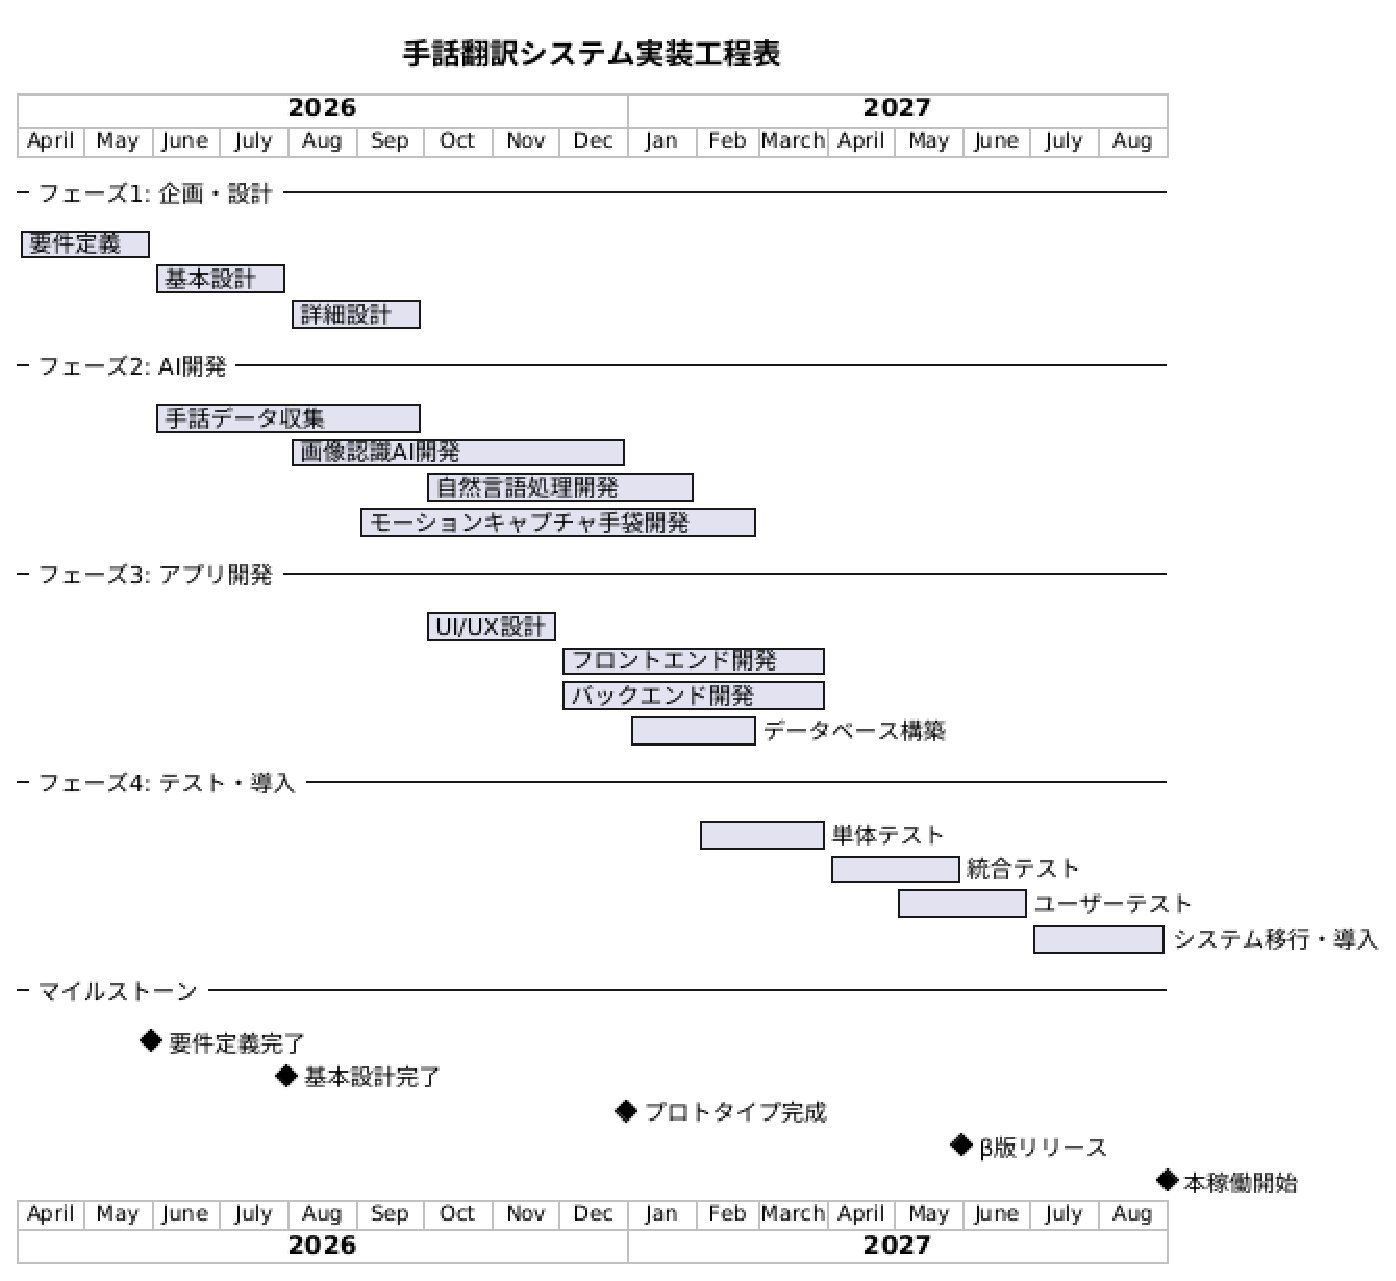
\includegraphics[width=\textwidth]{gantchart.eps}
\caption{手話翻訳システム実装工程表(2026年4月-2027年8月)}
\label{fig:gantchart}
\end{figure}

\section{効果}


\section{ポンチ絵(システム概要図)}


\section{まとめ}

\end{document}